\documentclass{article}
\usepackage[T1]{fontenc}
\usepackage{titlesec}
\usepackage{graphicx}
\usepackage{amsmath}
\usepackage{xcolor}
\usepackage{amssymb}
\usepackage{circuitikz}
\usepackage{trace}
\titleformat{\section}  % which section command to format
  {\fontsize{10}{12}\bfseries} % format for whole line
  {\thesection} % how to show number
  {1em} % space between number and text
  {} % formatting for just the text
  [] % formatting for after the text
  \title{Logika Cyfrowa}
\author{Jakub Gałaszewski} 
\begin{document}
\maketitle
\section{Zaprojektuj obwód, który mnoży ośmiobitową liczbę przez 1, 2, 3 lub 4, w zależności od wartości dodatkowego wejścia wyboru. Możesz wykorzystywać znane z wykładu podstawowe układy kombinacyjne (ale nie multiplikator).}
\begin{center}
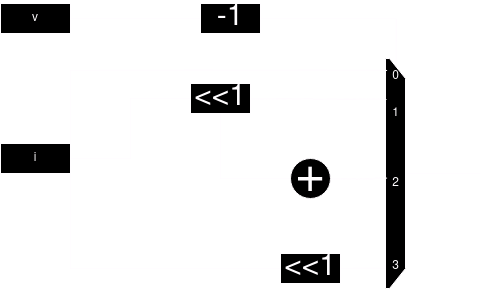
\includegraphics[scale=0.5]{./L05Z01.png}
\end{center}
\section{oniższy kod w SystemVerilogu miał implementować dekoder 2 do 4 z dodatkowym wejściem aktywującym, ale posiada błąd. Na czym on polega?}
\begin{center}
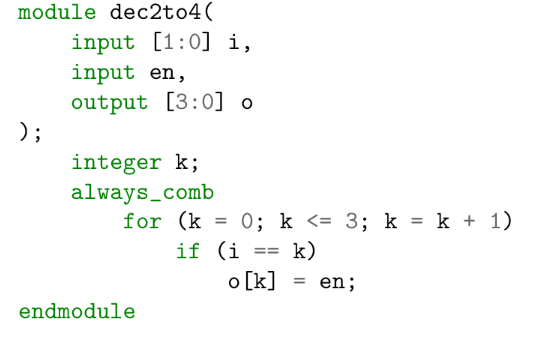
\includegraphics[scale=0.5]{./L05Z02.png}\\
UWAGA, output należy jeszcze ustalić na logic, czyli output logic [3:0]o
\end{center}
Problem jest (jeżeli dobrze zrozumiałem) że chcemy aby rozwiązane rozważało wszystkie gałęzie kodu, które są tutaj nierozpatrzone.
\section{Jaki obwód jest implementowany przez poniższy kod? Czy użyty styl implementacji jest tu dobrym wyborem?}
\begin{center}
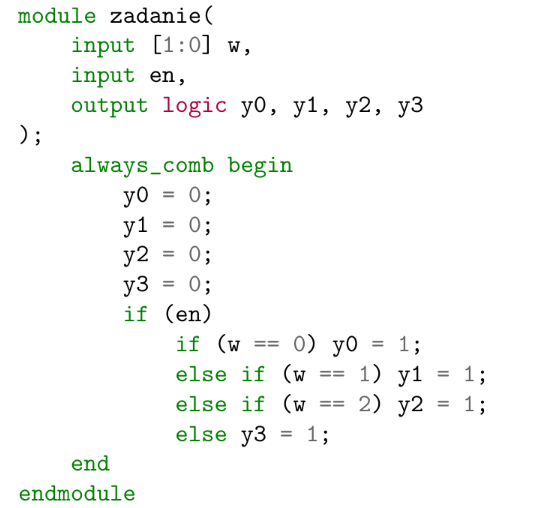
\includegraphics[scale=0.5]{./L05Z03.png}
\end{center}
jeżeli mamy bit en zapalony, to jest to dekoder 2 do 4, ale napisane w dosyć zawiłej formie. Wystarczy rozpisać kernaugha aby znacząco uprościć ten kod.
\begin{center}
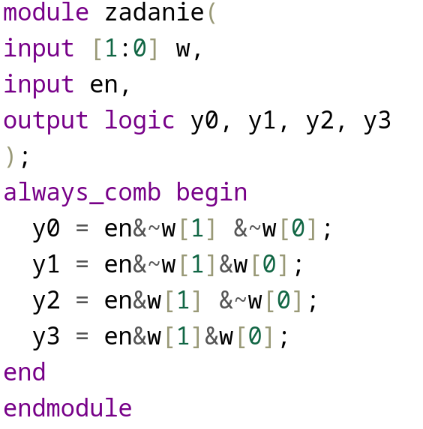
\includegraphics[scale=0.5]{./L05Z03v2.png}
\end{center}
\section{Pokaż, jak zaimplementować w SystemVerilogu dekoder 3 do 8 wykorzystując dwie instancje dekodera 2 do 4 z wejściem aktywującym i dodatkową logikę}
\begin{center}
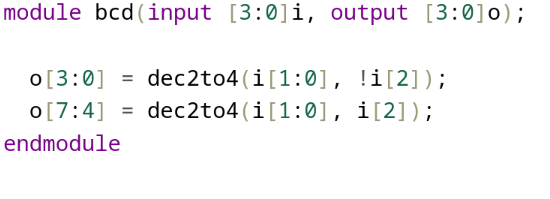
\includegraphics[scale=0.5]{./L05Z04v2.png}
\end{center}
\section{Wadą kodowania BCD jest skomplikowane obliczanie dopełnienia cyfry. Jednym z alternatywnych sposobów kodowania cyfr dziesiętnych jest kodowanie 8 4 -2 -1, w którym najmłodsze dwie cyfry binarne mają ujemne wagi. Zaimplementuj w SystemVerilogu konwerter kodowania cyfr z kodowania 8 4 -2 -1 do BCD.}
\begin{center}
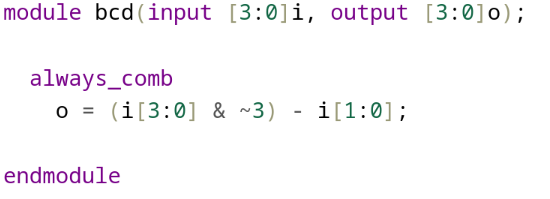
\includegraphics[scale=0.5]{./L05Z05.png}
\end{center}
\end{document}